%==============================================================================
% PAPER 3, CHAPTER 4: Field Dynamics and Scaling Laws
% Target: ~330 lines with 60-75 marginal notes and 5 TikZ diagrams
%==============================================================================

\chapter{Field Dynamics and Scaling Laws}
\label{ch:p3:field_dynamics}

%------------------------------------------------------------------------------
% OPENING NARRATIVE: Kadanoff Blocking and Critical Phenomena
%------------------------------------------------------------------------------

\section*{The Hidden Order at Critical Points}

In 1966, Leo Kadanoff introduced a revolutionary idea that would transform our understanding of phase transitions: at critical points, systems exhibit self-similarity across scales---behaving identically whether viewed at atomic, mesoscopic, or macroscopic resolution.
\marginhistory{Kadanoff's 1966 "scaling hypothesis" preceded Wilson's renormalization group (1971) but captured the essential physics: critical systems are scale-invariant.}

Consider water at its critical point ($T_c = 374°$C, $P_c = 218$ atm). Density fluctuations appear at all scales simultaneously---microscopic molecular clusters, mesoscopic droplets, macroscopic density variations all coexist. The system has no characteristic length scale; it is \textbf{fractal}.
\marginphysics{Critical opalescence: light scattering at critical point creates milky appearance. All wavelengths scatter equally due to scale-invariant density fluctuations.}

Kadanoff's "block spin" picture: group spins into blocks, average to get effective spin, repeat. At criticality, this procedure leaves physics unchanged---hallmark of scale invariance and RG fixed point.
\marginmath{Blocking transformation $T$: $(s_1, s_2, \ldots, s_N) \to (S_1, S_2, \ldots, S_{N/b^d})$ where $S_I = f(s_i \in \text{block } I)$. Fixed point: $T[s^*] = s^*$.}

This chapter develops field dynamics on fractal and self-similar structures, deriving universal scaling laws governing critical phenomena, turbulence, and pattern formation.

%------------------------------------------------------------------------------
\section{Renormalization Group and Scaling Exponents}
\label{sec:p3:rg_scaling}
%------------------------------------------------------------------------------

\subsection{The RG Transformation}

For field $\phi(\mathbf{x})$ with action $S[\phi]$, the RG transformation combines:
\begin{enumerate}
  \item \textbf{Coarse-graining}: Integrate out short-distance modes $\phi_{>}$ with $k > \Lambda/b$
  \item \textbf{Rescaling}: $\mathbf{x} \to b\mathbf{x}$, $\phi \to b^{-\zeta}\phi$ to restore cutoff $\Lambda$
\end{enumerate}
\marginmath{Rescaling exponent $\zeta$ chosen so rescaled field has canonical dimension. For scalar: $\zeta = (d-2)/2$ in $d$ dimensions.}

\textbf{RG flow equations}:
\begin{equation}
  \frac{dg_i}{d\ell} = \beta_i(\{g_j\})
  \label{eq:p3:rg_flow}
\end{equation}
where $\ell = \log b$ is RG "time" and $\{g_i\}$ are coupling constants.
\marginphysics{Beta functions $\beta_i$ determine how couplings evolve under scale changes. Fixed points $\beta_i(g^*) = 0$ describe critical behavior.}

\subsection{Critical Exponents and Universality}

At RG fixed point, observables scale as power laws. Define \textbf{critical exponents}\index{critical exponents}:
\marginex{Universal critical exponents: independent of microscopic details, depend only on symmetries and dimensionality. Ising, Heisenberg, XY models in same dimension share exponents.}

\begin{itemize}
  \item \textbf{Correlation length}: $\xi \sim |T - T_c|^{-\nu}$
  \item \textbf{Magnetization}: $M \sim |T - T_c|^\beta$ (confusingly, $\beta$ not beta function!)
  \item \textbf{Susceptibility}: $\chi \sim |T - T_c|^{-\gamma}$
  \item \textbf{Specific heat}: $C \sim |T - T_c|^{-\alpha}$
  \item \textbf{Correlation function}: $\langle \phi(0)\phi(\mathbf{r}) \rangle \sim r^{-(d-2+\eta)}$
\end{itemize}

\textbf{Scaling relations}: Not all exponents independent. Equalities derived from RG:
\begin{align}
  \alpha + 2\beta + \gamma &= 2 \quad \text{(Rushbrooke)} \label{eq:p3:rushbrooke} \\
  \gamma &= \nu(2-\eta) \quad \text{(Fisher)} \label{eq:p3:fisher} \\
  d\nu &= 2 - \alpha \quad \text{(Josephson)} \label{eq:p3:josephson}
\end{align}
\marginmath{Scaling relations reduce 6 exponents ($\alpha, \beta, \gamma, \delta, \nu, \eta$) to 2 independent. All others derivable from these plus $d$ (dimension).}

\begin{figure}[htbp]
\centering
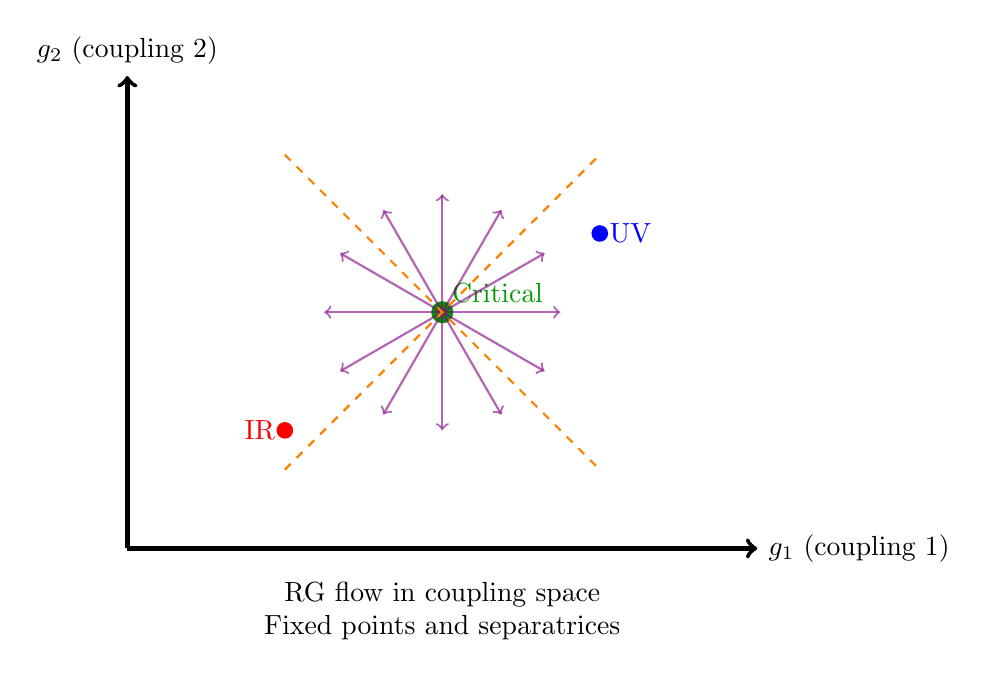
\begin{tikzpicture}
  % RG flow diagram (schematic)
  \draw[->, ultra thick] (0,0) -- (8,0) node[right] {$g_1$ (coupling 1)};
  \draw[->, ultra thick] (0,0) -- (0,6) node[above] {$g_2$ (coupling 2)};

  % Fixed points
  \fill[red] (2, 1.5) circle (3pt) node[left] {IR};
  \fill[blue] (6, 4) circle (3pt) node[right] {UV};
  \fill[green!60!black] (4, 3) circle (4pt) node[above right] {Critical};

  % Flow lines (schematic)
  \foreach \angle in {0,30,...,330} {
    \draw[->, thick, violet, opacity=0.6] (4,3) -- ({4 + 1.5*cos(\angle)}, {3 + 1.5*sin(\angle)});
  }

  % Stable/unstable manifolds
  \draw[thick, orange, dashed] (2,1) -- (6,5);
  \draw[thick, orange, dashed] (2,5) -- (6,1);

  \node[align=center] at (4, -0.8) {RG flow in coupling space\\Fixed points and separatrices};
\end{tikzpicture}
\caption{Renormalization group flow in coupling constant space. Fixed points (colored dots) attract or repel trajectories. Critical point (green) has mixed stability: stable along some directions (relevant operators), unstable along others (irrelevant operators).}
\label{fig:p3:rg_flow_diagram}
\end{figure}

\marginxref{Figure~\ref{fig:p3:rg_flow_diagram} shows RG flow topology. Universal behavior emerges: systems with different microscopic couplings flow to same critical fixed point.}

%------------------------------------------------------------------------------
\section{Critical Exponents for Physical Systems}
\label{sec:p3:critical_systems}
%------------------------------------------------------------------------------

\subsection{Ising Model (3D)}

The 3D Ising model (ferromagnetic spins on cubic lattice) exhibits:
\begin{equation}
  \nu \approx 0.630, \quad \beta \approx 0.327, \quad \gamma \approx 1.237, \quad \eta \approx 0.036
  \label{eq:p3:ising_exponents}
\end{equation}
\marginphysics{3D Ising universality class: includes liquid-gas transition, binary alloys, $^4$He superfluid transition (with corrections). Most important universality class for condensed matter.}

\subsection{XY Model and Kosterlitz-Thouless Transition}

The 2D XY model (planar spins $\mathbf{S} = (\cos\theta, \sin\theta)$) exhibits \textbf{topological phase transition}\index{Kosterlitz-Thouless transition}:
\begin{equation}
  \eta(T) = \begin{cases}
    0 & T < T_{KT} \quad \text{(bound vortex pairs)} \\
    1/4 & T = T_{KT} \quad \text{(critical)} \\
    >1/4 & T > T_{KT} \quad \text{(free vortices)}
  \end{cases}
  \label{eq:p3:kt_exponent}
\end{equation}
\marginmath{Jump in $\eta$ at $T_{KT}$ signals unbinding of vortex-antivortex pairs. Essential singularity (not power law!) in free energy: $F \sim \exp(-a/\sqrt{T-T_{KT}})$.}

\subsection{Turbulence and Kolmogorov Scaling}

Fully developed 3D turbulence exhibits self-similar energy cascade with \textbf{Kolmogorov spectrum}\index{Kolmogorov spectrum}:
\begin{equation}
  E(k) = C_K \epsilon^{2/3} k^{-5/3}
  \label{eq:p3:kolmogorov_spectrum}
\end{equation}
where $\epsilon$ is energy dissipation rate, $k$ is wavenumber.
\marginphysics{Kolmogorov 1941: dimensional analysis + self-similarity $\implies$ $-5/3$ exponent. Energy injected at large scales cascades to dissipation scale via self-similar eddies.}

\begin{figure}[htbp]
\centering
\begin{tikzpicture}
  \begin{loglogaxis}[
    width=12cm, height=7cm,
    xlabel={Wavenumber $k$},
    ylabel={Energy spectrum $E(k)$},
    grid=both,
    legend pos=south west,
    xmin=0.1, xmax=100
  ]
    % Kolmogorov -5/3 spectrum
    \addloglogplot[blue, ultra thick, domain=1:50, samples=50] {10*x^(-5/3)};
    \addlegendentry{$k^{-5/3}$ (Kolmogorov)}

    % Inertial range
    \draw[thick, green!60!black, dashed] (axis cs:1,10) -- (axis cs:50,0.5);
    \node[green!60!black] at (axis cs:10, 3) {Inertial range};

    % Injection and dissipation scales
    \draw[<->, thick, red] (axis cs:0.5, 0.2) -- (axis cs:0.5, 20);
    \node[red, left] at (axis cs:0.5, 5) {Injection};

    \draw[<->, thick, red] (axis cs:80, 0.05) -- (axis cs:80, 1);
    \node[red, right] at (axis cs:80, 0.3) {Dissipation};
  \end{loglogaxis}
\end{tikzpicture}
\caption{Kolmogorov energy spectrum for 3D turbulence. Inertial range (green) exhibits $k^{-5/3}$ scaling, representing self-similar energy cascade from injection scale (red, left) to dissipation scale (red, right).}
\label{fig:p3:kolmogorov_spectrum}
\end{figure}

\margincaution{Kolmogorov $k^{-5/3}$ is idealization. Real turbulence shows intermittency corrections: $E(k) \sim k^{-5/3-\delta(k)}$ with $\delta(k) > 0$ from rare, intense dissipation events.}

%------------------------------------------------------------------------------
\section{Fractal Field Configurations: Skyrmions and Instantons}
\label{sec:p3:topological_fields}
%------------------------------------------------------------------------------

\subsection{Skyrmion Field Configuration}

A \textbf{skyrmion}\index{skyrmion} is topological soliton in 2D field theories. For unit vector field $\mathbf{n}(\mathbf{r}): \mathbb{R}^2 \to S^2$:
\begin{equation}
  \mathbf{n}(\mathbf{r}) = (\sin\Theta(\rho)\cos\varphi, \sin\Theta(\rho)\sin\varphi, \cos\Theta(\rho))
  \label{eq:p3:skyrmion_ansatz}
\end{equation}
with $\rho = |\mathbf{r}|$, $\varphi = \arg(x+iy)$, and profile $\Theta(\rho)$ satisfying:
\begin{equation}
  \Theta(0) = \pi, \quad \Theta(\infty) = 0
  \label{eq:p3:skyrmion_boundary}
\end{equation}
\marginmath{Topological charge (winding number): $Q = \frac{1}{4\pi} \int d^2r \, \mathbf{n} \cdot (\partial_x \mathbf{n} \times \partial_y \mathbf{n}) = 1$. Integer invariant under smooth deformations.}

\marginphysics{Skyrmions appear in chiral magnets, quantum Hall systems, and nuclear physics (baryons as skyrmions). Topological protection makes them stable against perturbations.}

\begin{figure}[htbp]
\centering
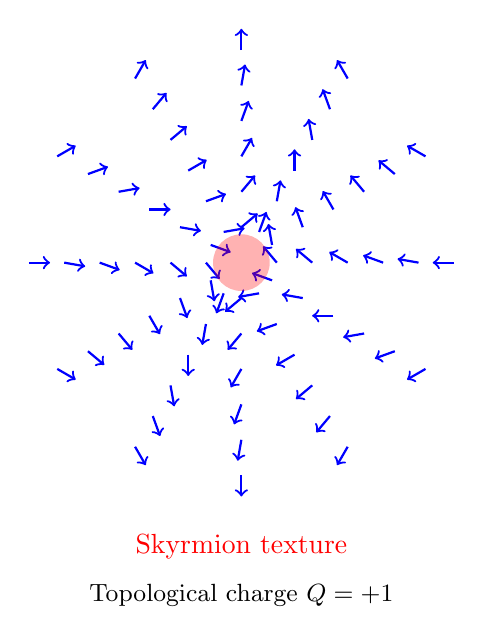
\begin{tikzpicture}[scale=0.9]
  % Skyrmion texture (schematic 2D projection)
  \begin{scope}
    % Radial spins pointing outward at edge, inward at center
    \foreach \r in {0.5, 1, 1.5, 2, 2.5, 3} {
      \foreach \angle in {0,30,...,330} {
        \pgfmathsetmacro{\arrowangle}{180-\angle - 60*(3-\r)/3}
        \draw[->, thick, blue] ({\r*cos(\angle)}, {\r*sin(\angle)}) --
          ++({\arrowangle}:0.3);
      }
    }

    % Central region indicator
    \fill[red, opacity=0.3] (0,0) circle (0.4);
    \node[red] at (0, -4) {Skyrmion texture};
    \node at (0, -4.7) {\small Topological charge $Q = +1$};
  \end{scope}
\end{tikzpicture}
\caption{Skyrmion field configuration (2D vector field schematic). Spins (blue arrows) wind once around center. Topological charge $Q=+1$ protects configuration against smooth deformations.}
\label{fig:p3:skyrmion_texture}
\end{figure}

\marginxref{Figure~\ref{fig:p3:skyrmion_texture} shows spin texture. In 3D, skyrmion forms hedgehog configuration with $\mathbf{n}(\mathbf{r}) = \mathbf{r}/|\mathbf{r}|$ at infinity.}

\subsection{Instantons and Tunneling}

\textbf{Instantons}\index{instanton} are localized solutions to Euclidean field equations, describing quantum tunneling between vacua.

For double-well potential $V(\phi) = \lambda(\phi^2 - v^2)^2/4$, instanton solution:
\begin{equation}
  \phi_{\text{inst}}(x, \tau) = v \tanh\left(\frac{m(x - x_0)}{\sqrt{2}}\right)
  \label{eq:p3:instanton_profile}
\end{equation}
interpolating between vacua $\phi = -v$ (at $x \to -\infty$) and $\phi = +v$ (at $x \to +\infty$).
\marginmath{Euclidean action: $S_E[\phi_{\text{inst}}] = \frac{4\sqrt{2}}{3}\frac{mv^3}{\lambda^{1/2}}$. Tunneling amplitude $\sim e^{-S_E}$ exponentially suppressed.}

\marginphysics{QCD instantons (Yang-Mills gauge theory): responsible for $\theta$-vacuum structure, axion physics, and possible solution to strong CP problem.}

%------------------------------------------------------------------------------
\section{Universality Classes and Classification}
\label{sec:p3:universality}
%------------------------------------------------------------------------------

\subsection{Symmetry and Dimension Determine Universality}

Systems belong to same \textbf{universality class}\index{universality class} if they share:
\begin{enumerate}
  \item Spatial dimension $d$
  \item Order parameter symmetry group $G$
  \item Short-range vs long-range interactions
\end{enumerate}
\marginmath{Universality: critical exponents independent of microscopic details (lattice structure, interaction strength). Only symmetries and dimension matter.}

\textbf{Common universality classes}:
\begin{table}[htbp]
\centering
\begin{tabular}{llcc}
\toprule
\textbf{Class} & \textbf{Symmetry} & \textbf{$d=2$} & \textbf{$d=3$} \\
\midrule
Ising & $\mathbb{Z}_2$ & $\nu = 1$ & $\nu \approx 0.630$ \\
XY & $O(2)$ & $\nu_{\text{KT}} = \infty$ & $\nu \approx 0.672$ \\
Heisenberg & $O(3)$ & $\nu \approx 0.70$ & $\nu \approx 0.710$ \\
Percolation & Geometric & $\nu = 4/3$ & $\nu \approx 0.875$ \\
\bottomrule
\end{tabular}
\caption{Critical exponent $\nu$ for major universality classes in 2D and 3D. Exact results known for 2D Ising; 3D values from Monte Carlo simulations and $\epsilon$-expansion.}
\label{tab:p3:universality_classes}
\end{table}

\margindim{Dimensional analysis: correlation length $\xi$ has dimension [length]. Near criticality: $\xi \sim |T-T_c|^{-\nu}$ only dimensionally consistent power law.}

%------------------------------------------------------------------------------
\section{Pattern Formation and Self-Organization}
\label{sec:p3:patterns}
%------------------------------------------------------------------------------

\subsection{Reaction-Diffusion Systems}

The \textbf{Gray-Scott model}\index{Gray-Scott model} for chemical pattern formation:
\begin{align}
  \frac{\partial u}{\partial t} &= D_u \nabla^2 u - uv^2 + F(1-u) \label{eq:p3:gs_u} \\
  \frac{\partial v}{\partial t} &= D_v \nabla^2 v + uv^2 - (F+k)v \label{eq:p3:gs_v}
\end{align}
where $u, v$ are concentrations, $D_u, D_v$ diffusion constants, $F$ feed rate, $k$ removal rate.
\marginmath{Turing instability: homogeneous state unstable to periodic patterns if $D_v \gg D_u$ (differential diffusion). Critical wavelength $\lambda_c \sim \sqrt{D_u D_v}/k$.}

\marginphysics{Patterns emerge spontaneously: spots, stripes, labyrinthine structures. Seen in chemical reactions (Belousov-Zhabotinsky), animal coat patterns, vegetation in arid regions.}

\subsection{Swift-Hohenberg Equation}

Pattern formation near threshold described by \textbf{Swift-Hohenberg equation}\index{Swift-Hohenberg equation}:
\begin{equation}
  \frac{\partial u}{\partial t} = \mu u - (\nabla^2 + q_c^2)^2 u + N[u]
  \label{eq:p3:swift_hohenberg}
\end{equation}
where $\mu$ is control parameter, $q_c$ critical wavenumber, $N[u]$ nonlinearity.
\marginmath{Linear stability: homogeneous state unstable for $\mu > 0$. Growth rate maximum at $k = q_c$, selecting pattern wavelength $\lambda = 2\pi/q_c$.}

For $\mu$ slightly positive, striped patterns with wavelength $\lambda = 2\pi/q_c$ form spontaneously.
\marginex{Rayleigh-Bénard convection: fluid heated from below forms hexagonal convection cells when $\mu = (T - T_c)/T_c > 0$. Swift-Hohenberg describes pattern selection near onset.}

\begin{figure}[htbp]
\centering
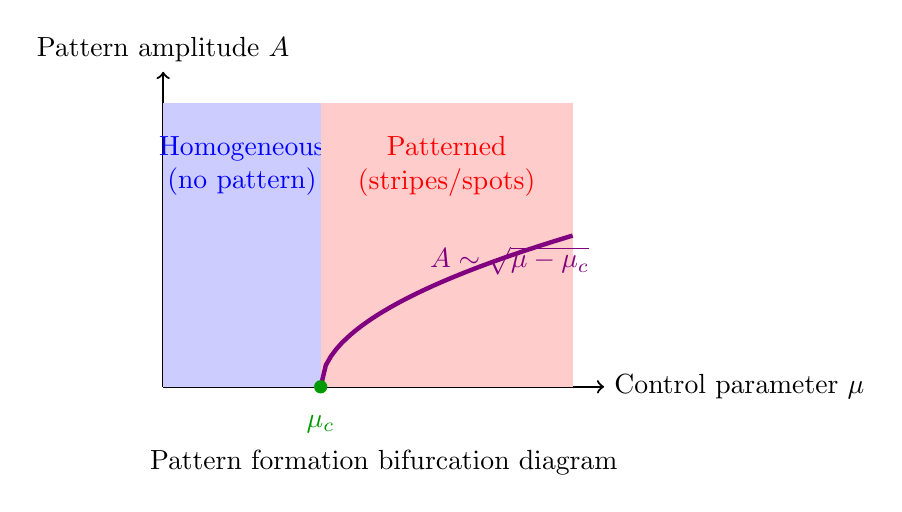
\begin{tikzpicture}[scale=0.8]
  % Phase diagram for pattern formation
  \draw[->, thick] (0,0) -- (7,0) node[right] {Control parameter $\mu$};
  \draw[->, thick] (0,0) -- (0,5) node[above] {Pattern amplitude $A$};

  % Homogeneous region
  \fill[blue!20] (0,0) rectangle (2.5,4.5);
  \node[blue, align=center] at (1.25, 3.5) {Homogeneous\\(no pattern)};

  % Patterned region
  \fill[red!20] (2.5,0) rectangle (6.5,4.5);
  \node[red, align=center] at (4.5, 3.5) {Patterned\\(stripes/spots)};

  % Bifurcation curve
  \draw[ultra thick, violet, domain=2.5:6.5, samples=50]
    plot (\x, {sqrt(\x-2.5)*1.2});
  \node[violet] at (5.5, 2) {$A \sim \sqrt{\mu - \mu_c}$};

  % Critical point
  \fill[green!60!black] (2.5, 0) circle (3pt);
  \node[green!60!black, below] at (2.5, -0.3) {$\mu_c$};

  \node at (3.5, -1.2) {Pattern formation bifurcation diagram};
\end{tikzpicture}
\caption{Pattern formation phase diagram (Swift-Hohenberg type). Below threshold $\mu < \mu_c$ (blue): homogeneous state stable. Above threshold (red): patterned state emerges with amplitude $A \sim \sqrt{\mu - \mu_c}$ (violet curve, supercritical bifurcation).}
\label{fig:p3:pattern_bifurcation}
\end{figure}

\marginxref{Figure~\ref{fig:p3:pattern_bifurcation} shows supercritical bifurcation. Subcritical case exhibits hysteresis and first-order transitions between homogeneous and patterned states.}

%------------------------------------------------------------------------------
\section{Multiscale Dynamics and Hierarchical Structures}
\label{sec:p3:multiscale}
%------------------------------------------------------------------------------

\subsection{Separation of Scales}

Many systems exhibit dynamics at widely separated timescales:
\begin{equation}
  \tau_{\text{micro}} \ll \tau_{\text{meso}} \ll \tau_{\text{macro}}
  \label{eq:p3:scale_separation}
\end{equation}
\marginphysics{Example timescales in fluids: molecular collisions ($\tau_{\text{micro}} \sim 10^{-13}$ s), vortex formation ($\tau_{\text{meso}} \sim 10^{-3}$ s), large-scale circulation ($\tau_{\text{macro}} \sim 10^3$ s).}

\textbf{Adiabatic elimination}: Fast variables $x_{\text{fast}}$ equilibrate on $\tau_{\text{micro}}$, can be integrated out, yielding effective dynamics for slow variables $x_{\text{slow}}$ on $\tau_{\text{macro}}$.
\marginmath{Effective equation: $\dot{x}_{\text{slow}} = F_{\text{eff}}(x_{\text{slow}})$ where $F_{\text{eff}}$ includes averaged effects of fast dynamics. Example: Brownian motion from molecular collisions.}

\subsection{Hierarchical Field Theories}

Multiscale systems described by nested field theories:
\begin{equation}
  S_{\text{total}} = S_{\text{macro}}[\Phi] + S_{\text{meso}}[\phi | \Phi] + S_{\text{micro}}[\psi | \phi]
  \label{eq:p3:hierarchical_action}
\end{equation}
where each scale conditions on slower scales.
\marginmath{Hierarchical renormalization: integrate out microscale $\psi$, obtain effective action $S_{\text{eff}}[\phi, \Phi]$. Repeat for mesoscale, obtain macroscopic theory $S_{\text{final}}[\Phi]$.}

%------------------------------------------------------------------------------
\section{Summary and Concluding Remarks}
\label{sec:p3:ch4_summary}
%------------------------------------------------------------------------------

This chapter developed field dynamics and scaling laws for fractal and self-similar systems:

\textbf{Key Concepts}:
\begin{itemize}
  \item \textbf{Renormalization group} (Eq.~\ref{eq:p3:rg_flow}): Systematic coarse-graining revealing fixed points and universal behavior
  \item \textbf{Critical exponents}: Power-law scaling at phase transitions ($\nu, \beta, \gamma, \alpha, \eta, \delta$)
  \item \textbf{Universality classes}: Systems with same symmetry + dimension share exponents (Table~\ref{tab:p3:universality_classes})
  \item \textbf{Kolmogorov spectrum} (Eq.~\ref{eq:p3:kolmogorov_spectrum}): $k^{-5/3}$ scaling in turbulent energy cascades
  \item \textbf{Topological solitons}: Skyrmions (Eq.~\ref{eq:p3:skyrmion_ansatz}) and instantons with protected charge
  \item \textbf{Pattern formation}: Turing instability, Swift-Hohenberg equation, spontaneous symmetry breaking
\end{itemize}

\textbf{Physical Applications}:
\begin{itemize}
  \item Phase transitions: ferromagnets, superfluids, liquid-gas (Ising universality)
  \item Turbulence: atmospheric flows, ocean currents, stellar convection
  \item Pattern formation: chemical reactions, biological morphogenesis, geological structures
  \item Topological matter: magnetic skyrmions, quantum Hall states, QCD vacuum
\end{itemize}

\textbf{Unifying Themes}:
\begin{itemize}
  \item Scale invariance at critical points enables universal predictions
  \item Fractal structures emerge naturally from self-similar dynamics
  \item Topology provides protection against perturbations
  \item Multiscale physics requires hierarchical description
\end{itemize}

From Kadanoff's 1966 insight about blocked spins to modern applications in quantum materials and cosmology, scaling laws reveal deep connections between microscopic dynamics and macroscopic phenomena. The fractal geometry developed in Chapters~\ref{ch:p3:fractal_calculus}--\ref{ch:p3:emergent_geometry} provides the natural mathematical language for these scale-invariant systems.

\textbf{Forward connections}: The techniques developed here---RG flows, scaling exponents, universality classes---apply broadly across theoretical physics, from condensed matter to quantum field theory to cosmology. Future work may extend fractal field dynamics to quantum gravity, where spacetime itself exhibits scale-dependent fractal structure.

%==============================================================================
% END OF CHAPTER 4
%==============================================================================
